\chapter{Opracowanie wyników}

Rozdział ten zawiera analizę wyników działania programu opisanego w~części~\ref{cha:implementacja}. Przeprowadzono także weryfikację wpływu usunięcia pojedynczego posterunku opadowego na uzyskane wskazanie opadowe na obszarze, co było jednym z~celów tej pracy.

\section{Warianty opadu}
Opisany w~rozdziale~\ref{cha:implementacja} program został uruchomiony celem wyznaczenia wartości opadu powierzchniowego dla obu przygotowanych wariantów funkcji opadowej. Poniżej zaprezentowano uzyskane wyniki.

\begin{table}[!ht]
\caption{Wyniki działania programu}
\begin{center}
\begin{tabular}{|c|c|c|c|}
\hline
 Wariant      & Opad wyznaczony [$m^3$] & Opad rzeczywisty [$m^3$] & Różnica [\%] \\ \hline \hline

 Paraboliczny & 1 462 995 563.4253  &   1 500 568 329.7155  &  -2.5039 \\ \hline
 Wymierny     & 1 559 081 843.8972  &   1 571 689 381.8665  &  -0.8022 \\ \hline

\end{tabular}
\end{center}
\end{table}

Jak można zauważyć, dla wariantu z~opadem parabolicznym mamy do czynienia z~niedomiarem. Jest to spodziewana sytuacja wynikająca z~interpolowania funkcji wklęsłej. Różnica z~rzeczywistą objętością opadu wynosi ok. 2.5\%, zatem jest to zadowalający wynik.

W przypadku wymiernego opadu uzyskano jeszcze lepsze wyniki. Błąd wyznaczonej wartości jest mniejszy niż jeden procent, a~należy zwrócić uwagę, iż dane przygotowane na potrzeby testów obejmują obszar rzędu stu tysięcy kilometrów kwadratowych.



\section{Analiza wrażliwości na posterunki opadowe}
W~tej części przeprowadzono wpływ wyłączenia wskazanego posterunku opadowego (ograniczono się do wybory punktów zawartych w granicach wskazanej zlewni) na wynik działania omawianej metody. Pozwala to znaleźć odpowiedź na pytanie: \textit{Czy sieć istniejących posterunków opadowych jest wystarczająca?}, a~to pomoże podejmować decyzje o~zwiększaniu ilości owych posterunków bądź przeniesieniu w~inną lokalizację.


Rysunek~\ref{fig:numery_posterunkow} przedstawia identyfikatory wykluczanych z~analizy punktów, natomiast wiersze poniższych tabel prezentują rezultaty działania programu bez zadanego punktu. Wartość wpływu usunięcia posterunku określona została względem wyznaczonego opadu powierzchniowego z~użyciem wszystkich punktów.

\begin{figure}[!ht]
	\centering
	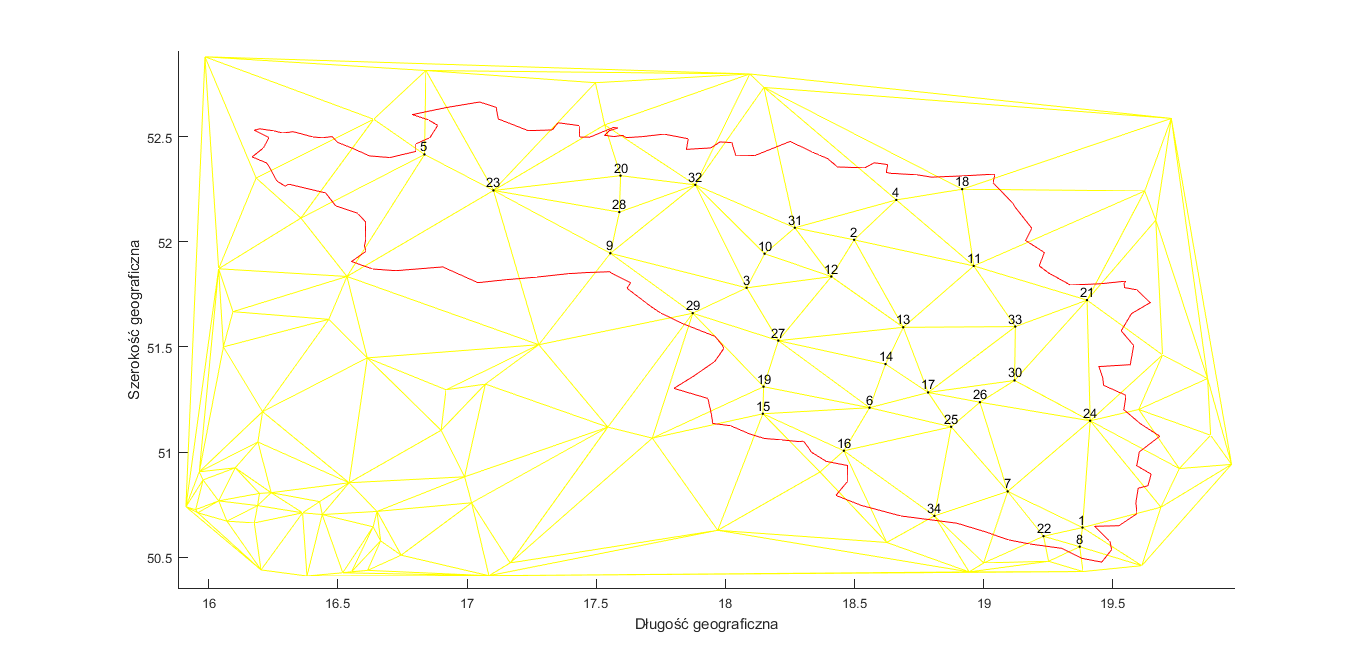
\includegraphics[width=1\linewidth]{identyfikatory_punktow}
	\caption{Identyfikatory posterunków wewnątrz zlewni}
	\label{fig:numery_posterunkow}
\end{figure}


%\subsection{Opad paraboliczny}

\begin{center}
\begin{longtable}{|c|c|c|c|r@{.}l|r@{.}l|}
\caption{Wpływ usunięcia posterunku na wynik algorytmu. Wariant paraboliczny.}\\

%nagłówek tabeli
\cline{2-3} \cline{5-8}
\multicolumn{1}{l}{} & \multicolumn{2}{|c|}{Opad $[m^3]$} & \multicolumn{1}{c}{} & \multicolumn{4}{|c|}{Wpływ posterunku} \\
\hline ID & Wyznaczony & Rzeczywisty & \multicolumn{1}{c}{Różnica [\%]} & \multicolumn{2}{|c|}{[$m^3$]}& \multicolumn{2}{|c|}{$\times 10^{-3} [\%]$} \\ \hline \hline
\hline
\endfirsthead


\multicolumn{8}{c}%
{\tablename\ \thetable\ -- \textit{Ciąg dalszy}} \\
\cline{2-3} \cline{5-8}
\multicolumn{1}{l}{} & \multicolumn{2}{|c|}{Opad $[m^3]$} & \multicolumn{1}{c}{} & \multicolumn{4}{|c|}{Wpływ posterunku} \\
\hline ID & Wyznaczony & Rzeczywisty & \multicolumn{1}{c}{Różnica [\%]} & \multicolumn{2}{|c|}{[$m^3$]}& \multicolumn{2}{|c|}{$\times 10^{-3} [\%]$} \\ \hline \hline
\hline
\endhead

\hline \multicolumn{8}{r}{\textit{Ciąg dalszy na następnej stronie}} \\
\endfoot
\hline
\endlastfoot
--  &     1 462 995 563.4253   &    1 500568329.7155   &      -2.5039  &                0 & 00     &     0 & 00 \\ \hline
1   &     1 463 076 745.5247   &    1 500568302.6776   &      -2.4984  &           81 182 & 0994   &     5 & 55 \\ \hline
2   &     1 461 776 787.8979   &    1 500568329.7155   &      -2.5851  &       -1 218 775 & 5274   &   -83 & 31 \\ \hline
3   &     1 462 473 733.6675   &    1 500568329.7155   &      -2.5386  &         -521 829 & 7578   &   -35 & 67 \\ \hline
4   &     1 460 378 875.6103   &    1 500568329.7155   &      -2.6782  &       -2 616 687 & 8150   &  -178 & 86 \\ \hline
5   &     1 468 988 504.7170   &    1 500568343.3016   &      -2.1045  &        5 992 941 & 2917   &   409 & 64 \\ \hline
6   &     1 461 622 417.1231   &    1 500568329.7155   &      -2.5954  &       -1 373 146 & 3022   &   -93 & 86 \\ \hline
7   &     1 464 682 183.9039   &    1 500568361.4533   &      -2.3915  &        1 686 620 & 4786   &   115 & 29 \\ \hline
8   &     1 462 995 563.4253   &    1 500568329.7155   &      -2.5039  &               -0 & 0000   &     0 & 00 \\ \hline
9   &     1 453 656 531.6541   &    1 500568329.7155   &      -3.1262  &       -9 339 031 & 7712   &  -638 & 35 \\ \hline
10  &     1 462 338 580.8233   &    1 500568329.7155   &      -2.5476  &         -656 982 & 6020   &   -44 & 91 \\ \hline
11  &     1 454 316 634.1198   &    1 500568329.7155   &      -3.0822  &       -8 678 929 & 3055   &  -593 & 23 \\ \hline
12  &     1 460 880 307.4094   &    1 500568329.7155   &      -2.6448  &       -2 115 256 & 0159   &  -144 & 58 \\ \hline
13  &     1 460 206 170.9554   &    1 500568329.7155   &      -2.6897  &       -2 789 392 & 4699   &  -190 & 66 \\ \hline
14  &     1 461 450 430.2504   &    1 500568329.7155   &      -2.6068  &       -1 545 133 & 1749   &  -105 & 61 \\ \hline
15  &     1 462 002 685.7047   &    1 500568329.7155   &      -2.5700  &         -992 877 & 7206   &   -67 & 87 \\ \hline
16  &     1 462 214 551.1240   &    1 500568329.7155   &      -2.5559  &         -781 012 & 3013   &   -53 & 38 \\ \hline
17  &     1 462 691 315.1618   &    1 500568329.7155   &      -2.5241  &         -304 248 & 2635   &   -20 & 80 \\ \hline
18  &     1 464 582 760.9851   &    1 500568329.7155   &      -2.3981  &        1 587 197 & 5598   &   108 & 49 \\ \hline
19  &     1 461 064 560.9566   &    1 500568329.7155   &      -2.6325  &       -1 931 002 & 4687   &  -131 & 99 \\ \hline
20  &     1 461 310 691.7342   &    1 500568329.7155   &      -2.6161  &       -1 684 871 & 6911   &  -115 & 17 \\ \hline
21  &     1 459 561 769.3807   &    1 500568329.7155   &      -2.7327  &       -3 433 794 & 0446   &  -234 & 71 \\ \hline
22  &     1 463 418 751.6247   &    1 500568331.6960   &      -2.4757  &          423 188 & 1994   &   -28 & 93 \\ \hline
23  &     1 453 767 799.3651   &    1 500568329.7155   &      -3.1189  &       -9 227 764 & 0602   &  -630 & 74 \\ \hline
24  &     1 462 113 590.3990   &    1 500568331.1793   &      -2.5627  &         -881 973 & 0263   &   -60 & 29 \\ \hline
25  &     1 461 120 846.7018   &    1 500568329.7155   &      -2.6288  &       -1 874 716 & 7235   &  -128 & 14 \\ \hline
26  &     1 462 704 787.1648   &    1 500568329.7155   &      -2.5233  &         -290 776 & 2605   &   -19 & 88 \\ \hline
27  &     1 460 220 263.7528   &    1 500568329.7155   &      -2.6889  &       -2 775 299 & 6725   &  -189 & 70 \\ \hline
28  &     1 461 578 202.4715   &    1 500568329.7155   &      -2.5984  &       -1 417 360 & 9538   &   -96 & 88 \\ \hline
29  &     1 461 321 743.5352   &    1 500568329.7155   &      -2.6154  &       -1 673 819 & 8901   &  -114 & 41 \\ \hline
30  &     1 460 813 336.2660   &    1 500568329.7155   &      -2.6493  &       -2 182 227 & 1593   &  -149 & 16 \\ \hline
31  &     1 460 877 238.9356   &    1 500568329.7155   &      -2.6451  &       -2 118 324 & 4897   &  -144 & 79 \\ \hline
32  &     1 461 214 840.5295   &    1 500568329.7155   &      -2.6226  &       -1 780 722 & 8958   &  -121 & 72 \\ \hline
33  &     1 460 597 607.6173   &    1 500568329.7155   &      -2.6637  &       -2 397 955 & 8080   &  -163 & 91 \\ \hline
34  &     1 462 056 933.3298   &    1 500568329.7155   &      -2.5665  &         -938 630 & 0955   &   -64 & 16 \\ \hline
\end{longtable}
\end{center}




%\subsection{Opad wymierny}

\begin{center}
\begin{longtable}{|c|c|c|c|r@{.}l|r@{.}l|}
\caption{Wpływ usunięcia posterunku na wynik algorytmu. Wariant wymierny.}\\

%nagłówek tabeli
\cline{2-3} \cline{5-8}
\multicolumn{1}{l}{} & \multicolumn{2}{|c|}{Opad $[m^3]$} & \multicolumn{1}{c}{} & \multicolumn{4}{|c|}{Wpływ posterunku} \\
\hline ID & Wyznaczony & Rzeczywisty & \multicolumn{1}{c}{Różnica [\%]} & \multicolumn{2}{|c|}{[$m^3$]}& \multicolumn{2}{|c|}{$\times 10^{-3} [\%]$} \\ \hline \hline
\hline
\endfirsthead


\multicolumn{8}{c}%
{\tablename\ \thetable\ -- \textit{Ciąg dalszy}} \\
\cline{2-3} \cline{5-8}
\multicolumn{1}{l}{} & \multicolumn{2}{|c|}{Opad $[m^3]$} & \multicolumn{1}{c}{} & \multicolumn{4}{|c|}{Wpływ posterunku} \\
\hline ID & Wyznaczony & Rzeczywisty & \multicolumn{1}{c}{Różnica [\%]} & \multicolumn{2}{|c|}{[$m^3$]}& \multicolumn{2}{|c|}{$\times 10^{-3} [\%]$} \\ \hline \hline
\hline
\endhead

\hline \multicolumn{8}{r}{\textit{Ciąg dalszy na następnej stronie}} \\
\endfoot
\hline
\endlastfoot

%DANE
0  &  1 559 081 843.8972  & 1 571 689 381.8665   &  -0.8022  &           0 & 0     &     0 & 0    \\ \hline
1  &  1 559 061 775.4774  & 1 571 689 381.8665   &  -0.8034  &     -20 068 & 4198  &    -1 & 2872 \\ \hline
2  &  1 559 556 499.2791  & 1 571 689 381.8665   &  -0.7720  &     474 655 & 3819  &    30 & 4445 \\ \hline
3  &  1 559 136 538.3012  & 1 571 689 381.8665   &  -0.7987  &      54 694 & 4040  &     3 & 5081 \\ \hline
4  &  1 559 442 692.3556  & 1 571 689 381.8665   &  -0.7792  &     360 848 & 4584  &    23 & 1449 \\ \hline
5  &  1 559 947 406.5283  & 1 571 689 417.0476   &  -0.7471  &     865 562 & 6311  &    55 & 5175 \\ \hline
6  &  1 558 176 477.3967  & 1 571 689 381.8665   &  -0.8598  &    -905 366 & 5004  &   -58 & 0705 \\ \hline
7  &  1 560 786 375.3441  & 1 571 689 381.8665   &  -0.6937  &   1 704 531 & 4469  &   109 & 3292 \\ \hline
8  &  1 559 095 618.9713  & 1 571 689 381.8665   &  -0.8013  &      13 775 & 0741  &     0 & 8835 \\ \hline
9  &  1 552 651 800.4294  & 1 571 689 381.8665   &  -1.2113  &  -6 430 043 & 4678  &  -412 & 4250 \\ \hline
10 &  1 558 714 645.8784  & 1 571 689 381.8666   &  -0.8255  &    -367 198 & 0188  &   -23 & 5522 \\ \hline
11 &  1 554 874 657.8980  & 1 571 689 381.8665   &  -1.0699  &  -4 207 185 & 9992  &  -269 & 8502 \\ \hline
12 &  1 557 211 624.0194  & 1 571 689 381.8665   &  -0.9212  &  -1 870 219 & 8778  &  -119 & 9565 \\ \hline
13 &  1 554 450 898.6458  & 1 571 689 381.8665   &  -1.0968  &  -4 630 945 & 2514  &  -297 & 0303 \\ \hline
14 &  1 556 565 978.0968  & 1 571 689 381.8665   &  -0.9622  &  -2 515 865 & 8004  &  -161 & 3684 \\ \hline
15 &  1 558 917 063.7066  & 1 571 689 381.8665   &  -0.8126  &    -164 780 & 1905  &   -10 & 5691 \\ \hline
16 &  1 558 885 218.0005  & 1 571 689 381.8665   &  -0.8147  &    -196 625 & 8967  &   -12 & 6116 \\ \hline
17 &  1 559 015 351.5139  & 1 571 689 381.8665   &  -0.8064  &     -66 492 & 3833  &    -4 & 2648 \\ \hline
18 &  1 559 633 185.1938  & 1 571 689 381.8665   &  -0.7671  &     551 341 & 2966  &    35 & 3632 \\ \hline
19 &  1 555 968 588.0481  & 1 571 689 381.8665   &  -1.0002  &  -3 113 255 & 8491  &  -199 & 6852 \\ \hline
20 &  1 560 044 700.0865  & 1 571 689 381.8665   &  -0.7409  &     962 856 & 1894  &    61 & 7579 \\ \hline
21 &  1 558 107 108.7750  & 1 571 689 381.8665   &  -0.8642  &    -974 735 & 1222  &   -62 & 5198 \\ \hline
22 &  1 559 169 427.6163  & 1 571 689 381.8665   &  -0.7966  &      87 583 & 7191  &     5 & 6176 \\ \hline
23 &  1 559 280 152.8309  & 1 571 689 381.8665   &  -0.7895  &     198 308 & 9338  &    12 & 7196 \\ \hline
24 &  1 559 105 231.7239  & 1 571 689 381.8665   &  -0.8007  &      23 387 & 8267  &     1 & 5001 \\ \hline
25 &  1 559 151 654.4141  & 1 571 689 381.8665   &  -0.7977  &      69 810 & 5169  &     4 & 4777 \\ \hline
26 &  1 558 860 933.0753  & 1 571 689 381.8665   &  -0.8162  &    -220 910 & 8219  &   -14 & 1693 \\ \hline
27 &  1 555 324 767.4248  & 1 571 689 381.8665   &  -1.0412  &  -3 757 076 & 4723  &  -240 & 9801 \\ \hline
28 &  1 559 984 330.8331  & 1 571 689 381.8666   &  -0.7447  &     902 486 & 9359  &    57 & 8858 \\ \hline
29 &  1 557 620 436.7111  & 1 571 689 381.8665   &  -0.8951  &  -1 461 407 & 1861  &   -93 & 7351 \\ \hline
30 &  1 556 501 296.1849  & 1 571 689 381.8665   &  -0.9664  &  -2 580 547 & 7122  &  -165 & 5171 \\ \hline
31 &  1 559 981 653.3915  & 1 571 689 381.8665   &  -0.7449  &     899 809 & 4943  &    57 & 7141 \\ \hline
32 &  1 561 086 734.8301  & 1 571 689 381.8666   &  -0.6746  &   2 004 890 & 9329  &   128 & 5943 \\ \hline
33 &  1 557 739 362.4966  & 1 571 689 381.8665   &  -0.8876  &  -1 342 481 & 4006  &   -86 & 1072 \\ \hline
34 &  1 558 890 117.2658  & 1 571 689 381.8665   &  -0.8144  &    -191 726 & 6314  &   -12 & 2974 \\ \hline

\end{longtable}
\end{center}

Analizując wyniki dla wariantu parabolicznego można zauważyć, iż największy wpływ na zaburzenie wyniku miało usunięcie takich punktów jak 9, 11 i 23. Nie powinno to być niespodzianką, ponieważ zagęszczenie posterunków w~sąsiedztwie wyżej wymienionych jest niewielkie. Usunięcie ich powoduje pozostawienie obszaru o~stosunkowo dużej powierzchni bez stanowiska pomiarowego. Co tyczy się posterunków jak 1, 8 czy 18 - ich usunięcie nie wpływa na uzyskany wynik, a~nawet poprawia go. Takie rezultaty mogą być sygnałem dla osób odpowiedzialnych za rozmieszczenie posterunków do zwiększenia ich ilości na terenach z~deficytem urządzeń pomiarowych. Pokazują też, które z~nich (jak 1, 8, 17, 18 czy 22) można przenieść w~inne miejsce i~przyniesie to korzyści.


Wariant opadu określonego funkcją wymierną wykazuje mniejsze odchylenie rezultatu od wartości rzeczywistych. Wpływ wskazanych wyżej posterunków jest analogiczny i~w~tym przypadku co potwierdza poprawność działania narzędzia. Znaczne zwiększenie błędu powoduje usunięcie punktu numer 9~lub 11. Odnotowano większą wrażliwość na punkty 13 i~27, natomiast wykluczenie 23 spowodowało tutaj (minimalną) poprawę wyniku, przeciwnie do pierwszego wariantu.

Nie można pominąć faktu, iż podczas usuwania posterunków zaobserwowano różnice w~opadzie rzeczywistym wyliczonym opisaną w~części~\ref{sec:funkcje_opadu} metodą. Częstsze różnice obserwuje się dla wariantu opadu parabolicznego, czego powodem może być fakt spłaszczenia wspomnianej funkcji. Inną przyczyną może być generowanie trójkątów, które funkcja całkująca środowiska MatLab uważa za zbyt małe, stąd pewne odchylenie.

\section{Wielkość błędu}
Zaproponowane dane testowe to obszar obejmujący szerokości geograficzne od 50.41 do 52.88 (w~formacie dziesiętnym). Stosowany sposób konwersji współrzędnych geograficznych (wzór~\ref{eq:konwersja_wspolrzednych}) dla takich wartości generuje niedokładność długości jednego stopnia wynoszącą $\pm 1.88 km$. Należy zwrócić uwagę, iż niedokładność ta nie wpływa na działanie omawianego programu, ponieważ tak on, jak i~funkcje wyznaczające wartości opadu oraz pseudorzeczywistego opadu powierzchniowego opierają się na współrzędnych metrycznych, już po konwersji, natomiast dane wejściowe do programu zostały spreparowane.  

Wspomniane w~poprzednim podrozdziale niedokładności wyznaczonej wartości opadu powierzchniowego są zadowalające. Błąd względny w najgorszym przypadku wyniósł 3.08\%. Należy pamiętać, iż implementowane rozwiązanie miałoby być elementem składowym systemu alarmującego (który uwzględnia bufor bezpieczeństwa), wobec tego stuprocentowa dokładność nie jest jednym z wymagań.